\documentclass[serif,9pt]{beamer}
\usetheme{Boadilla}
\usepackage{color}
\definecolor{moradoInma}{rgb}{0.5,0,0.7}
\usecolortheme[named=moradoInma]{structure}

\usepackage[latin1]{inputenc}
\usepackage[spanish]{babel}
\usepackage{caption}
\usepackage{graphicx} % figuras
\usepackage{subfigure} % subfiguras
\usepackage{float}


\definecolor{dkgreen}{rgb}{0,0.6,0}
\definecolor{gray}{rgb}{0.5,0.5,0.5}
\definecolor{mauve}{rgb}{0.58,0,0.82}

\usepackage{listings}
\lstset
{ %Formatting for code in appendix
  language=C++, % choose the language of the code
  basicstyle=\footnotesize\color{black},
  keywordstyle=\color{moradoInma}\bfseries, % style for keywords
  numberstyle=\tiny, % the size of the fonts that are used for the line-numbers     
  backgroundcolor=\color{white},
  showspaces=false, % show spaces adding particular underscores
  showstringspaces=false, % underline spaces within strings
  showtabs=false, % show tabs within strings adding particular underscores
  tabsize=2, % sets default tabsize to 2 spaces
  captionpos=b, % sets the caption-position to bottom
  breaklines=false, % sets automatic line breaking
  breakatwhitespace=false, 
}

\restylefloat{figure}

\beamersetuncovermixins{\opaqueness<1>{25}}{\opaqueness<2->{15}}

\begin{document}

\title{Algoritmo Backtracking: Viajante de Comercio}  
\author{David Cabezas Berrido \\ Patricia C�rdoba Hidalgo \\ Emilio Jos� Hoyo Medina \\ Inmaculada Mar�n Carballo}
\date{\today}

\begin{frame}
\titlepage
\end{frame}

\begin{frame}\frametitle{Contenido}
\tableofcontents
\end{frame} 

\section{Problema} 

\subsection{Viajante de Comercio}

\begin{frame}[fragile]\frametitle{Viajante de Comercio} 
  El problema del viajante de comercio (TSP, por Traveling Salesman
  Problem): dado un conjunto de ciudades y una matriz con las
  distancias entre todas ellas, un viajante debe recorrer todas las
  ciudades exactamente una vez, regresando al punto de partida, de
  forma tal que la distancia recorrida sea m�nima.
\end{frame}

\section{Algoritmos}

\begin{frame}[fragile]{Funci�n cota}
  \begin{lstlisting}
  int weightBound(const vector<int> &visited, int currentWeight) const{
    int bound = currentWeight;

    for(int i = 1; i < n; i++)
      if(find(visited.begin(),visited.end(),i)==visited.end())
        bound += bestDistance(i);

    bound += bestDistance(visited.front());

    return bound;
  }
  \end{lstlisting}
\end{frame}

  \subsection{Backtracking}

  \begin{frame}[fragile]\frametitle{Backtracking} 
    \begin{lstlisting}
void backtracking(const TSP& tsp, const vector<int> &visited,
      vector<int> &bestSol, int currentWeight, int& minimumWeight){

  if(visited.size() == tsp.getN()){
    currentWeight += tsp.getDistance(visited.back(),visited.front());
    if(currentWeight < minimumWeight){
      minimumWeight = currentWeight;
      bestSol = visited;
    }
    return;
  }

  if(tsp.weightBound(visited, currentWeight) >= minimumWeight)
    return;

  int weight;
  vector<int> aux;

  for(int i = 1; i < tsp.getN(); i++){
    weight = currentWeight;
    aux = visited;
    if(find(visited.begin(),visited.end(),i)==visited.end()){
      aux.push_back(i);
      weight += tsp.getDistance(i,visited.back());
      backtracking(tsp, aux, bestSol, weight, minimumWeight);
    }
  }
}
\end{lstlisting}    
\end{frame}

\subsection{Branch and Bound}

\begin{frame}[fragile]\frametitle{Branch and Bound}

\begin{lstlisting}[basicstyle=\tiny]
  void BandB(const TSP& tsp, multiset<node> &alive_nodes, vector<int> &bestSol,
  int& minimumWeight, int &maxsize, int &expanded, int &pruned){

  if(alive_nodes.empty()) return;
  
  node n = *alive_nodes.begin();
  alive_nodes.erase(alive_nodes.begin());
  
  if(n.bound >= minimumWeight) return;

  if(n.visited.size() == tsp.getN()){
 
    n.currentWeight += tsp.getDistance(n.visited.front(), n.visited.back());

    if(n.currentWeight < minimumWeight){
      minimumWeight = n.currentWeight;
      bestSol = n.visited;
      pruned = prune(alive_nodes,minimumWeight);
    }
    BandB(tsp, alive_nodes, bestSol, minimumWeight, maxsize, expanded, pruned);
  }
  else { 
    node aux;
  
    for(int i = 1; i < tsp.getN(); i++){
      if(find(n.visited.begin(), n.visited.end(), i) == n.visited.end()){
        aux = n;
        aux.visited.push_back(i);
        aux.currentWeight += tsp.getDistance(i, n.visited.back());
        tsp.weightBound(aux.visited, aux.currentWeight);
        alive_nodes.insert(aux);
      }
    }

    BandB(tsp, alive_nodes, bestSol, minimumWeight, maxsize, expanded, pruned);
  }
}
\end{lstlisting}

\end{frame}

\section{Resultados emp�ricos}
\subsection{Eficiencia emp�rica}
\begin{frame}\frametitle{Eficiencia Backtracking}
\begin{figure}[H]
  \centering \subfigure{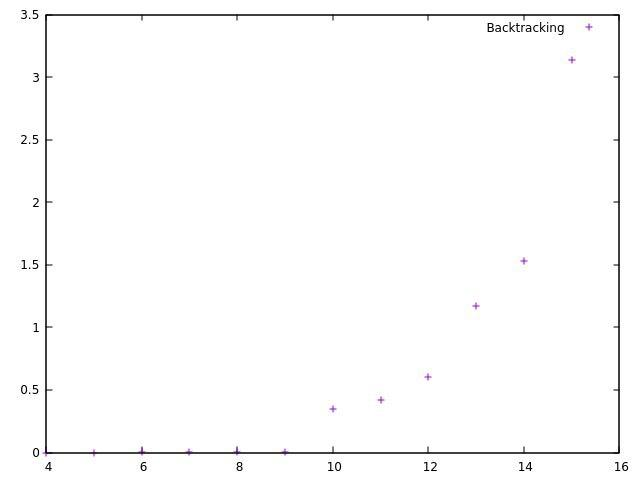
\includegraphics[width=70mm]{graficas/tiempos/backtracking}}
\end{figure}
\end{frame}

\begin{frame}\frametitle{Eficiencia B\&B}
\begin{figure}[H]
  \centering \subfigure{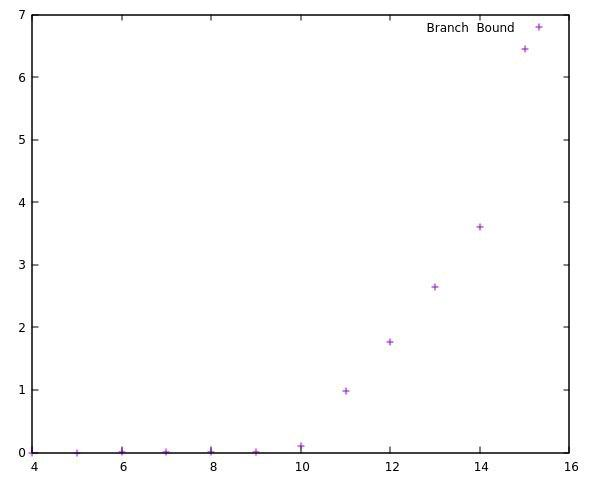
\includegraphics[width=70mm]{graficas/tiempos/B&B}}
\end{figure}
\end{frame}

\begin{frame}\frametitle{Comparaci�n}
  
  \begin{figure}[H]
  \centering \subfigure{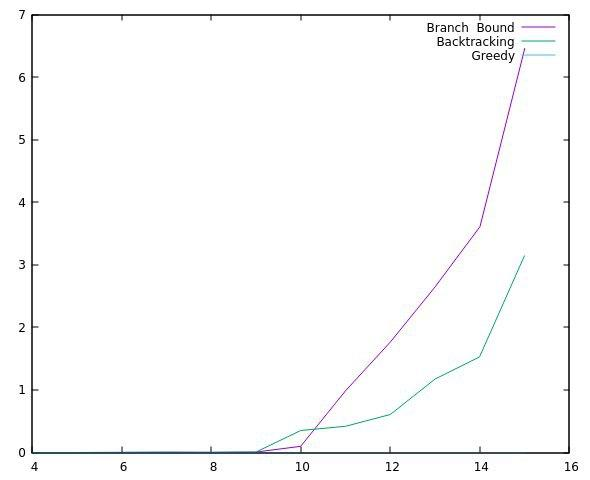
\includegraphics[width=70mm]{graficas/tiempos/comparacion}}
\end{figure}
\end{frame}

\subsection{Comparativa}

\begin{frame}\frametitle{Comparativa}
  \begin{table}[!hbp]
    \centering
    \label{tab:tiempos}
    \begin{tabular}{| c | c | c | c |}
      \hline
      \multicolumn{1}{|c|}{$\textbf{n}$}& \textbf{Backtracking}&\textbf{Branch and Bound}& \textbf{Greedy} \\ \hline
      4 & 5.7e-05    & 0.000104  & 6e-06     \\ 
      5 & 0.000229   & 0.000401  & 1.2e-05   \\ 
      6 & 0.000943   & 0.001835 & 1.8e-05   \\ 
      7 & 0.002449   & 0.004233 & 2.7e-05   \\ 
      8 & 0.001312   & 0.002789  & 3.5e-05   \\ 
      9 & 0.005933   & 0.006234  & 5e-05     \\ 
      10 & 0.350949  & 0.09896   & 6.7e-05   \\ 
      11 & 0.554521  & 0.98615   & 8.8e-05   \\ 
      12 & 0.857285  & 1.76516   & 0.000106  \\
      13 & 1.17463   & 2.64651  & 0.000131  \\
      14 & 1.52913   & 3.60603  & 0.000166  \\
      15 & 3.14079   & 6.45577   & 0.000202  \\ \hline
    \end{tabular}
  \end{table}
\end{frame}

\section{Conclusi�n}

\begin{frame}
  \huge CONCLUSI�N \\

  \begin{enumerate}
  \item Greedy: el m�s r�pido / soluci�n aproximada
  \item Backtracking: lento / soluci�n �ptima
  \item Branch \& Bound: lento / soluci�n �ptima
    \end{enumerate}
\end{frame}


\end{document}